\documentclass[a4paper, 11pt, oneside, openright, english]{book}
\usepackage[utf8]{inputenc}
\usepackage{graphicx}
\usepackage{hyperref}
\usepackage{booktabs}
\usepackage{blindtext}
\usepackage{amsmath}
\usepackage{amssymb}
\usepackage{listings}
\usepackage{titlesec}
\usepackage[usenames,dvipsnames]{xcolor}
\usepackage{longtable}
\usepackage{seqsplit}
\usepackage{geometry}
\usepackage{fancyhdr}
\usepackage{float}
\usepackage{enumitem}
\usepackage{array}
\usepackage{multicol}
\usepackage{caption}
\usepackage{listings}
\usepackage[T1]{fontenc}  % Use T1 font encoding
\usepackage{beramono}

% Define JavaScript language style
\lstdefinelanguage{JavaScript}{
    keywords={const, let, var, if, else, for, while, function},
    keywordstyle=\color{blue},
    commentstyle=\color{gray},
    stringstyle=\color{ForestGreen},
    morecomment=[l]{//},
    morecomment=[s]{/*}{*/},
    morestring=[b]",
    morestring=[b]'
}

% Define SQL language style
\lstdefinelanguage{SQL}{
    keywords={SELECT, FROM, WHERE, INSERT, INTO, VALUES, UPDATE, SET, DELETE, CREATE, TABLE, PRIMARY, KEY, REFERENCES, FOREIGN, ON, CASCADE, CONSTRAINT, CHECK, UNIQUE, NOT, NULL, AUTO_INCREMENT, ALTER, ADD, DROP, INDEX, DESC, ASC, LIMIT, OFFSET, JOIN, INNER, LEFT, RIGHT, OUTER, UNION, ALL, GROUP, BY, HAVING, ORDER, BY, AVG, SUM, COUNT, MAX, MIN, AS, OR, AND, IN, LIKE, BETWEEN, IS, NULL, TRUE, FALSE},
    keywordstyle=\color{orange},
    commentstyle=\color{BlueViolet},
    stringstyle=\color{ForestGreen},
    morecomment=[l]{--},
    morecomment=[s]{/*}{*/},
    morestring=[b]",
    morestring=[b]'
}

% Set general listings style
\lstset{
    basicstyle=\ttfamily\footnotesize,
    showstringspaces=false,
    tabsize=2,
    breaklines=true
}

\pagestyle{fancy}
\fancyhf{}

\fancyhead[LE,RO]{\slshape \rightmark}
\fancyhead[LO,RE]{\slshape \leftmark}
\fancyfoot[C]{\thepage}
\renewcommand{\chaptermark}[1]{\markboth{#1}{}}
\renewcommand{\sectionmark}[1]{\markright{\thesection.\ #1}}

\setlength{\headheight}{13.59999pt}
\addtolength{\topmargin}{-1.59999pt}

\titleformat{\chapter}[block]{\normalfont\huge\bfseries}{\thechapter.}{1em}{\Huge}

\begin{document}
\input title
\input revision_history
\tableofcontents

\chapter{Introduction}

\section{Purpose}

The purpose of the MLUD is to digitize and streamline the process of cataloging and monitoring the used schoolbook market held at Lokalino during the summer. The system aims to eeduce the workload on operators, particularly for repetitive tasks, minimize errors by eliminating manual transcription processes and significantly decrease paper usage.

\section{Scope}

The MLUD will be used by operators, providers and buyers. The system will allow operators to manage the catalog of books, providers to add books to the catalog and buyers to search for books. The system will also allow operators to account for the books sold and help the financial transactions between providers and buyers.
The system does not handle actual financial transactions but keeps a record of the money involved in the transactions.

\noindent The boundaries of the system are as follows:
\begin{itemize}
    \item Operations are limited to the Lokalino summer book market.
    \item The platform will only retain data for one year after market closure, except for users who opt into the mailing list.
\end{itemize}

\section{Definitions, acronyms and abbreviations}

\begin{table}[H]
    \centering
    \begin{tabular}{|l|l|l|}
        \hline
        \textbf{Term}   & \textbf{Definition}             & \textbf{Acronym} \\ \hline
        Operator        & A Lokalino employee             & OP               \\
        Provider        & A person who has books to sell  & PR               \\
        Buyer           & A person who wants to buy books & BY               \\
        Mercatino Libri & The system                      & MLUD             \\\hline
    \end{tabular}
\end{table} 
\chapter{Requirement Analysis and Specification}

The MLUD will offer the following functionalities:
\begin{itemize}
    \item User registration and book detail submission via an online form.
    \item Facilitating the physical handover of books, including verification and labeling.
    \item Streamlining the sales process with a digital interface for managing transactions.
    \item Tracking unsold books and managing financial settlements for sellers.
    \item Generating aggregated statistical reports to monitor performance and user satisfaction.
\end{itemize}

\section{Hardware Interfaces}
The system will be accessible through a web interface. The PR will have the option to use both a computer and a mobile device to access the system, so the interface must be responsive and usable on both platforms.

The OP will use a computer to access the system, so the interface must be optimized for computer use.

\section{Use Cases}

The use cases are illustrated in the diagram in Figure \ref{fig:use_cases}.

\begin{figure}[h]
    \centering
    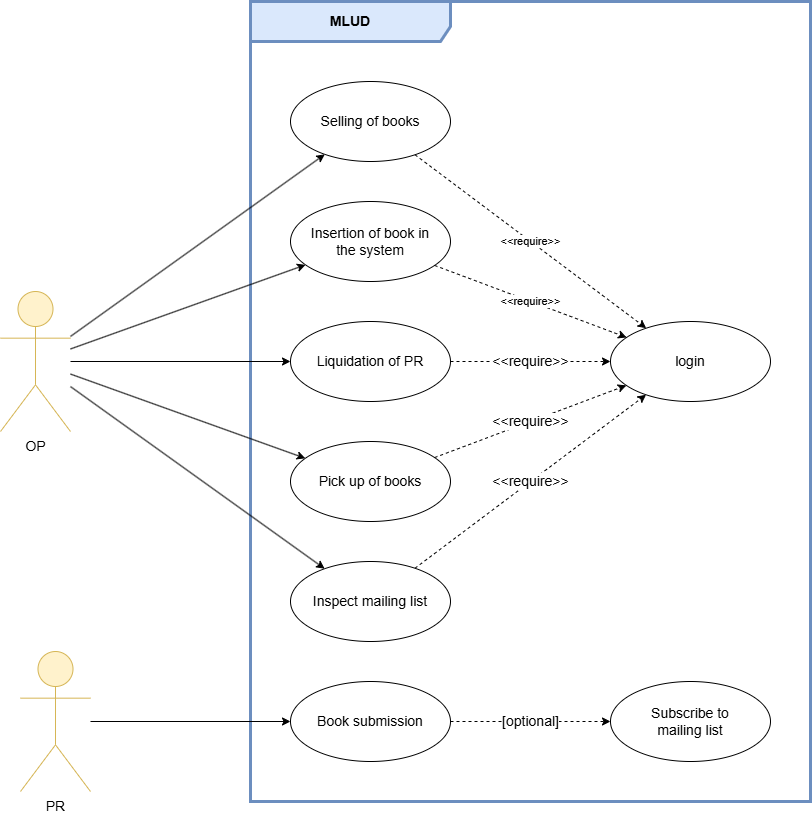
\includegraphics[width=.75\textwidth]{assets/use_cases_diagram.png}
    \caption{Use cases diagram}
    \label{fig:use_cases}
\end{figure}

\subsection{Use Case 1: Book submission}

\begin{enumerate}
    \item The PR accesses the system.
    \item The PR fills out the form, providing:
          \begin{itemize}
              \item Personal information (name, surname, email, phone number).
              \item Information for an arbitrary number of books (ISBN, title, author, edition, price, condition).
              \item Acceptance of the terms and conditions.
              \item Preference for subscription to the mailing list.
          \end{itemize}
          When entering the ISBN, the system will suggest the book's information if it is already in the system.
    \item The PR submits the form, it is redirected to a confirmation page and receives a confirmation email.
\end{enumerate}


\subsection{Use Case 2: Book delivery}

\begin{enumerate}
    \item The PR goes to Lokalino with the books.
    \item The OP accesses the protected area of the system.
    \item The OP searches for the record of the PR in the system.
    \item The OP verifies the correspondence between the books and the records, eventually updating the records or adding comments
    \item If all is correct, the OP labels the books to identify the corresponding PR
    \item The OP mark the correct delivery of the books in the system
\end{enumerate}

\subsection{Use Case 3: Book sale}

\begin{enumerate}
    \item The OP accesses the protected area of the system.
    \item The BY selects the books they want to buy.
    \item For each book, the OP searches for the record in the system and adds the book to the cart.
    \item At the end of the selection, the OP confirms the purchase and collects the payment. The books are marked as sold in the system.
\end{enumerate}

\subsection{Use Case 4: Liquidation and return of unsold books}

\begin{enumerate}
    \item The OP accesses the protected area of the system.
    \item The OP searches for the record of the PR in the system.
    \item The system shows the list of books unsold and the total amount due to the PR.
    \item The PR collects the money and the unsold books.
    \item The OP marks the books as returned in the system.
\end{enumerate}

\section{Special Requirements}

In order to facilitate the filling of the form by the PR, the system will provide a search function that will suggest the book's information when the ISBN is entered. In order to generate this suggestion, the system will also allow the OP to manually enter the book's information, possibly before the beginning of the event.

The system will keep the data of the PRs and the books for 1 year after the event, and after that, it will be deleted. The only data that will be kept indefinitely is the list of persons who have subscribed to the mailing list.

\section{Assumptions}
\label{sec:assumptions}

A couple of assumptions have been made in the design of the system:

\begin{itemize}
    \item Even if in the implementation every PR will be identified by a unique ID, the system will check the uniqueness of the email address; this comes into play when a PR submits the form: if the email address is already in the system and the PR fills out the form again, the system will not create a new record and will work as if the same PR is inserting more books.
    \item Same thing for the ISBN: if the ISBN is already in the system, the system will suggest the book's information, and the PR will not have to fill out the form for that book. If the PR wants to insert different informations for a book that is already in the system (for example, a different price, or a different author), the system will discard the data inputted by the PR and will use the data already in the system.
\end{itemize}
\chapter{Design}




\section{Component diagram}

The system will be organized in a classical client-server configuration, and the latter will expose RESTful APIs to the clients, and a web application for both OPs and PRs. Every service will be in its own servlet. The component diagram is shown in Figure \ref{fig:component}.

\begin{figure}[h]
    \centering
    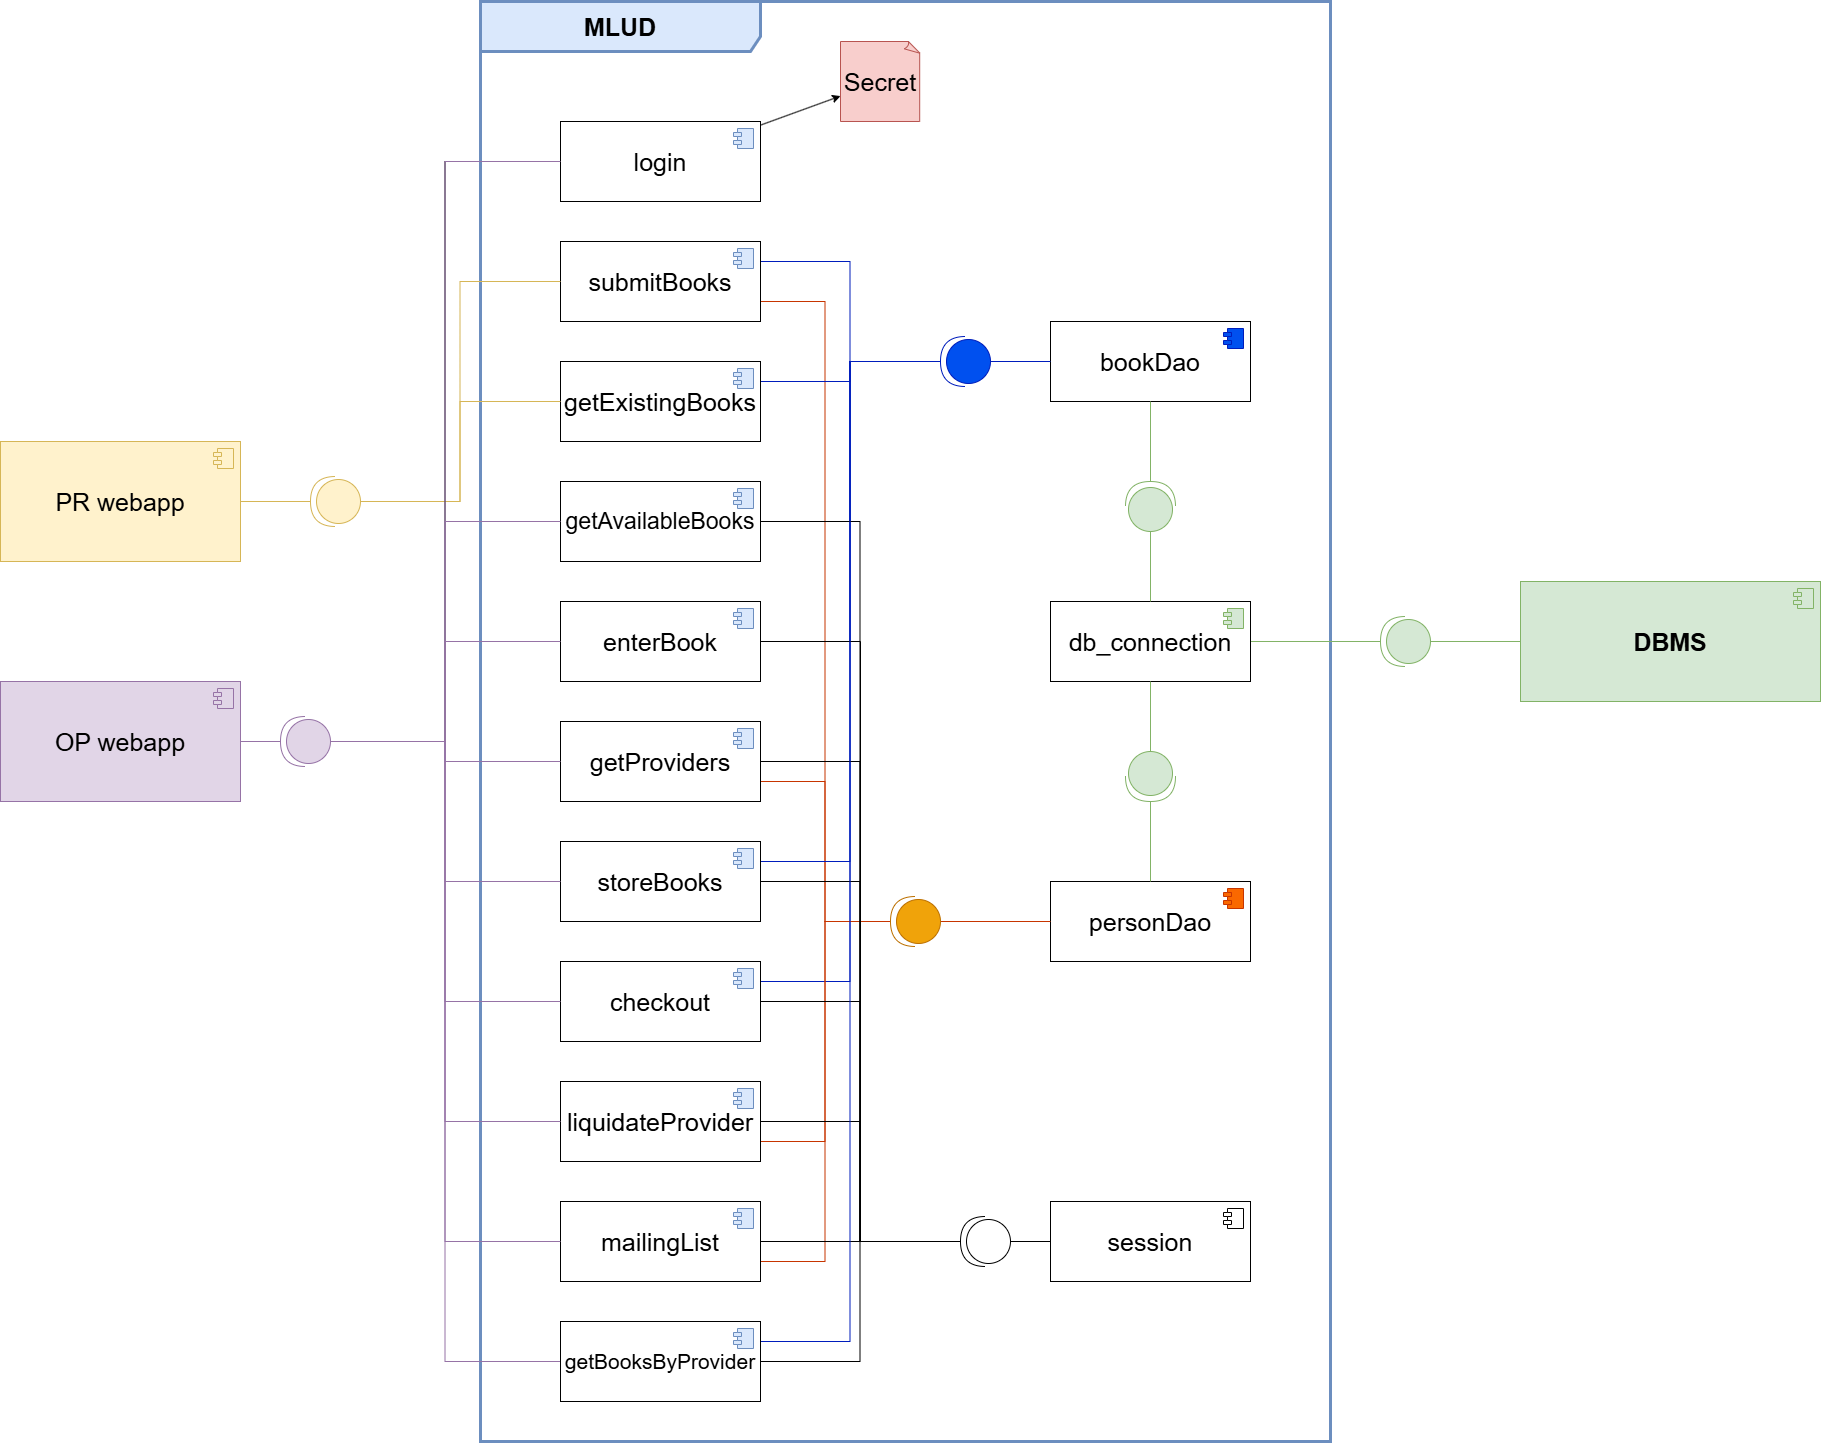
\includegraphics[width=\textwidth]{assets/component_diagram.png}
    \caption{Component diagram}
    \label{fig:component}
\end{figure}

\section{Logical description of data}

The data will be stored into a relational database, which will be designed according to the Logical schema in Figure \ref{fig:er}.

\begin{figure}[h]
    \centering
    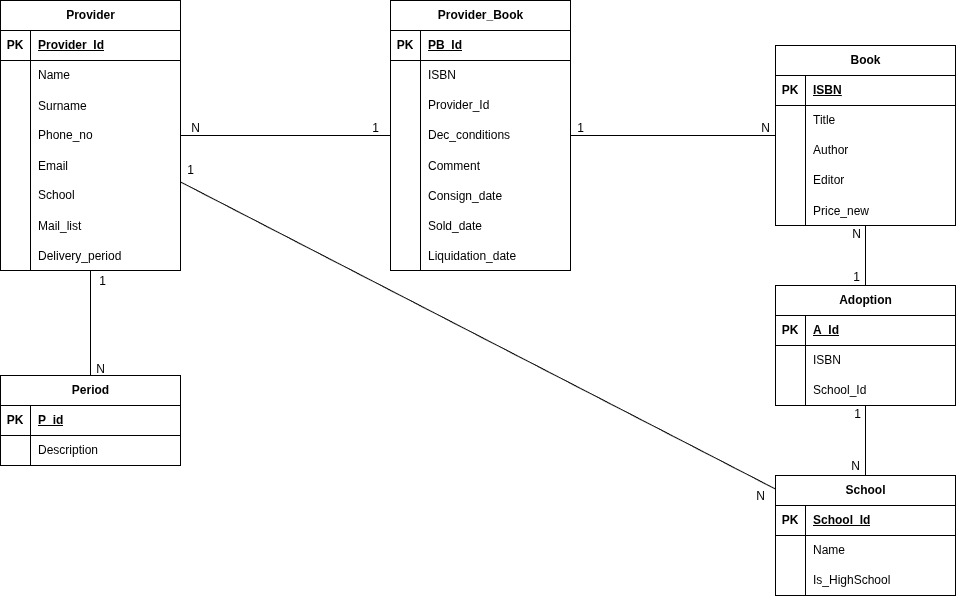
\includegraphics[width=\textwidth]{assets/er_diagram.png}
    \caption{Logical schema of the database}
    \label{fig:er}
\end{figure}

\section{API endpoints}

The API will expose the endpoints in a structure coherent with the compoenent diagram \ref{fig:component}. It follows a list of the endpoints:

\subsection{Login}
\textbf{Method} : POST \\
\textbf{EndPoint} : /login.php \\
\textbf{Body parameters} :
\begin{lstlisting}[language=JavaScript, label={lst:jscode}, basicstyle=\ttfamily]
{ "Hashed_password": String }
\end{lstlisting}
\textbf{Response} : \texttt{200} if the login is successful, \texttt{401} if the password is wrong.

\subsection{Submit Books}
A PR submits its books to the system, and gives its personal information.\\
\textbf{Method} : POST \\
\textbf{EndPoint} : /submitBooks.php \\
\textbf{Body parameters} :
\begin{lstlisting}[language=JavaScript, label={lst:jscode}, basicstyle=\ttfamily]
{
    "Name": String,
    "Surname": String,
    "School": String,
    "Email": String,
    "Phone": String,
    "Books": [
        {
            "ISBN": String,
            "Title": String,
            "Author": String,
            "Editor": String,
            "Price_new": Number,
            "Dec_conditions": String
        },
        ...
    ],
    "Mail_list": Boolean
}
\end{lstlisting}
\textbf{Response} : \texttt{200} if the submission is successful, \texttt{400} if the request is malformed.

\subsection{Get Existing Books}
The system returns the information of the books already in the system, searching by ISBN.\\
\textbf{Method} : GET \\
\textbf{EndPoint} : /getExistingBooks.php \\
\textbf{URL parameters} :
\begin{itemize}
    \item \texttt{ISBN}: String
\end{itemize}
\textbf{Response} :
\begin{lstlisting}[language=JavaScript, label={lst:jscode}, basicstyle=\ttfamily]
[
    {
        "ISBN": String,
        "Title": String,
        "Author": String,
        "Editor": String,
        "Price_new": Number
    },
    ...
]
\end{lstlisting}

\subsection{Get Books in Stock}
The system returns all the books in stock, i.e. the books both submitted and actually delivered by the PRs.\\
\textbf{Method} : GET \\
\textbf{EndPoint} : /getAvailableBooks.php \\
\textbf{Response} :
\begin{lstlisting}[language=JavaScript, label={lst:jscode}, basicstyle=\ttfamily]
[
    {
        "ISBN": String,
        "Title": String,
        "Author": String,
        "Editor": String,
        "Price_new": Number,
        "ProviderName": String,
        "ProviderSurname": String,
        "PB_Id": Number,
        "Provider_Id": Number,
        "Dec_conditions": String,
        "Comments"? : String,
        "Consign_date": String,
        % // didn't have the sbatta to remove them from the select
        "Sold_date": null, 
        "Liquidation_date": null

    },
    ...
]
\end{lstlisting}

\subsection{Enter book}
An OP enters a book in the system, associating it to a ISBN. No strong need for this, it's just to make simpler the PR submission.\\
\textbf{Method} : POST \\
\textbf{EndPoint} : /enterBook.php \\
\textbf{Body parameters} :
\begin{lstlisting}[language=JavaScript, label={lst:jscode}, basicstyle=\ttfamily]
{
    "ISBN": String,
    "Title": String,
    "Author": String,
    "Editor": String,
    "Price_new": Number
}
\end{lstlisting}
\textbf{Response} : \texttt{200} if the submission is successful, \texttt{400} if the request is malformed.

\subsection{Get PRs}
The system returns the list of PRs, to handle the delivery of the books and the liquidation.
\textbf{Method} : GET \\
\textbf{EndPoint} : /getProviders.php \\
\textbf{Response} :
\begin{lstlisting}[language=JavaScript, label={lst:jscode}, basicstyle=\ttfamily]
[
    {
        "Provider_Id": Number,
        "Name": String,
        "Surname": String,
        "State": String
    },
    ...
]
\end{lstlisting}
The possible states are:
\begin{itemize}
    \item \texttt{0} - waiting for delivery
    \item \texttt{1} - waiting for liquidation
    \item \texttt{2} - liquidated
\end{itemize}

\subsection{Deliver Books}
A PR delivers the books to the OP.\\
\textbf{Method} : POST \\
\textbf{EndPoint} : /storeBooks.php \\
\textbf{Body parameters} :
\begin{lstlisting}[language=JavaScript, label={lst:jscode}, basicstyle=\ttfamily]
[
    {
        "PB_Id": Number,
        "Comments"?: String
    },
    ...
]
\end{lstlisting}
\textbf{Response} : \texttt{200} if the submission is successful, \texttt{400} if the request is malformed.

\subsection{Sell Books}
An OP sells the books to a BY.\\
\textbf{Method} : POST \\
\textbf{EndPoint} : /sellBooks.php \\
\textbf{Body parameters} :
\begin{lstlisting}[language=JavaScript, label={lst:jscode}, basicstyle=\ttfamily]
[
    { "PB_Id": Number },
    ...
]
\end{lstlisting}
\textbf{Response} : \texttt{200} if the submission is successful, \texttt{400} if the request is malformed.

\subsection{Liquidate PR and return unsold books}
An OP liquidates the PR, returning the unsold books and the money.\\
\textbf{Method} : POST \\
\textbf{EndPoint} : /liquidateProvider.php \\
\textbf{Body parameters} :
\begin{lstlisting}[language=JavaScript, label={lst:jscode}, basicstyle=\ttfamily]
{ "Provider_Id": Number, }
\end{lstlisting}
\textbf{Response} : \texttt{200} if the submission is successful, \texttt{400} if the request is malformed.

\subsection{Mailing list}
Show the list of PRs that accepted to be in the mailing list.\\
\textbf{Method} : GET \\
\textbf{EndPoint} : /mailingList.php \\
\textbf{Response} :
\begin{lstlisting}[language=JavaScript, label={lst:jscode}, basicstyle=\ttfamily]
[
    {
        "Name": String,
        "Surname": String,
        "Email": String
    },
    ...
]
\end{lstlisting}


\section{Deployment}

All the webapp will be entirely deployed on the free hosting service \href{www.altervista.org}{Altervista}, which provides a MySQL database and a php server, so all the problems of deployment, reliability, scalability, and security are handled by the service provider.

\section{UX design}

The webapp will be designed with a simple and intuitive interface, with a clean and modern look.

The UX is explained at an high level in the flow diagrams in Figures \ref{fig:flow_book_submission} and \ref{fig:flow_op}.

\begin{figure}[ht]
    \centering
    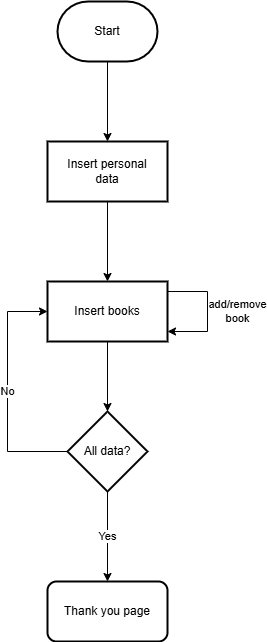
\includegraphics[width=.25\textwidth]{assets/flow_book_submission.png}
    \caption{Flow of the book submission}
    \label{fig:flow_book_submission}
\end{figure}

\begin{figure}[ht]
    \centering
    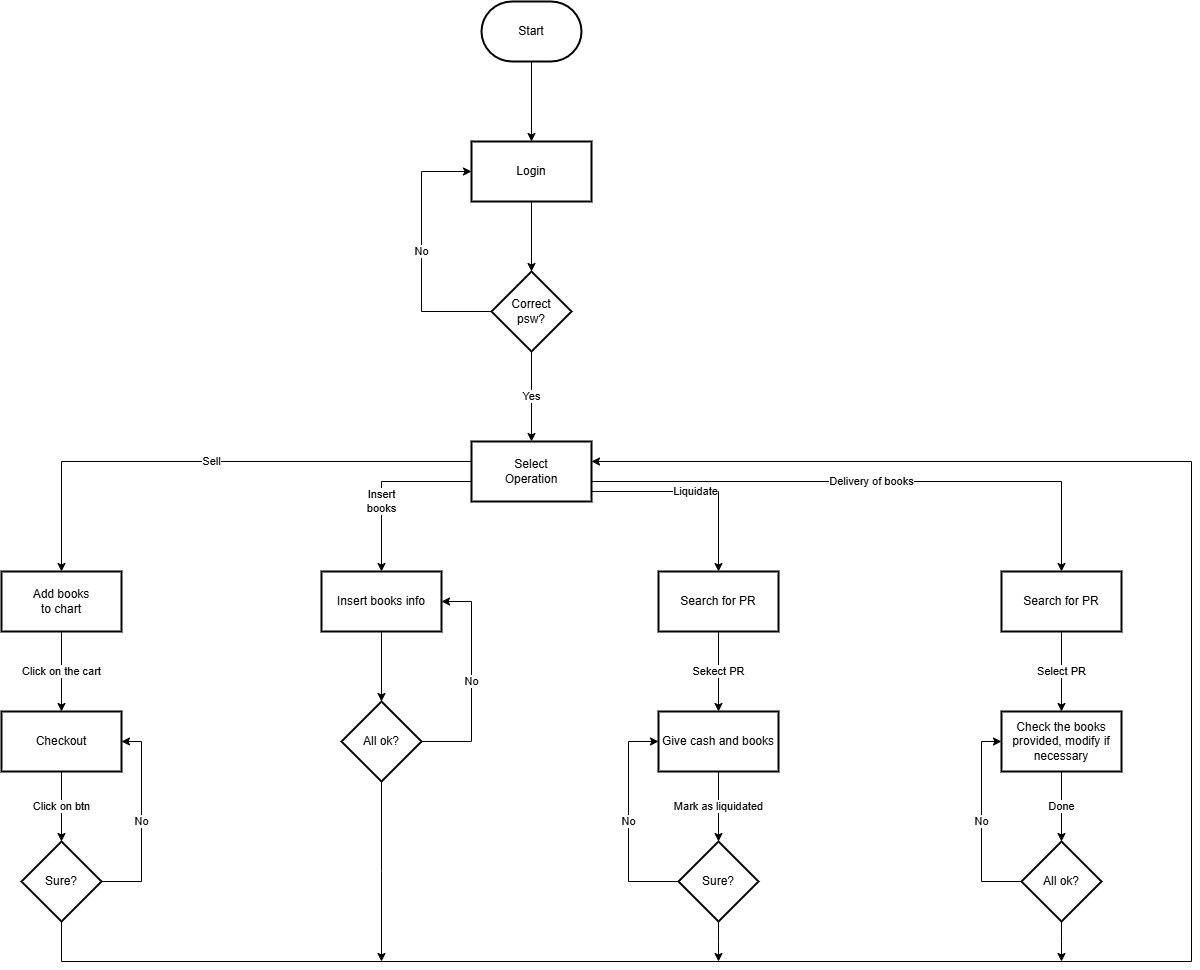
\includegraphics[width=\textwidth]{assets/flow_op.png}
    \caption{Flow of the OP}
    \label{fig:flow_op}
\end{figure}

\section{User interface}

Still WIP. Screenshots will be added in a future release of the document.
\chapter{Implementation}

All the code is open source under the \href{https://www.apache.org/licenses/LICENSE-2.0}{Apache 2.0 license} and can be found on GitHub at

\begin{center}    
    \url{https://github.com/pontig/lokalino_mlud}.
\end{center}

\section{Adopted development framework}

\subsection*{Backend}

The backend is implemented in \textbf{php}, since it is the language that the author is most familiar with and it is the only backend supported by Altervista (the free hosting service used for the project).

\subsection*{Frontend}

The frontend is implemented in \textbf{React}. React is a JavaScript library for building user interfaces. It is maintained by Facebook and a community of individual developers and companies. React can be used as a base in the development of single-page or mobile applications, since it is capable of handling the view layer for web and mobile apps. React was chosen because it is a modern and widely used library that allows for the creation of a dynamic and responsive user interface.

\section{Structure of the souece code}
The source code is structured in a way that separates the frontend from the backend, both organized in an intuitive way and easy to scale and maintain.

The full structure of the source code is as follows:
\begin{itemize}[label={}]
    \item \texttt{backend/} - contains the backend code
          \begin{itemize}[label={}]
              \item \texttt{dao/} - contains the data access objects, one for the books and one for the PR. it also contains the database connection
              \item \texttt{utils/} - contains the utility functions, such as the session management and the secret passwords of the OPs
              \item \texttt{*.php} - the servlets that handle the requests from the frontend
          \end{itemize}
    \item \texttt{frontend/} - contains the React application
          \begin{itemize}[label={}]
              \item \texttt{build/} - contains the compiled code (not included in the repository)
              \item \texttt{public/} - contains the static files, such as the index.html and the icons
              \item \texttt{src/} - contains the source code
                    \begin{itemize}[label={}]
                        \item \texttt{pages/} - contains the pages of the application
                        \item \texttt{styles/} - contains the stylesheets
                        \item \texttt{types/} - contains the typescript interfaces
                        \item \texttt{App.js} - the main component of the application
                        \item \texttt{index.js} - the entry point of the application
                    \end{itemize}
          \end{itemize}
\end{itemize}

\section{Test plan}

The testing of the application will be done once the development is complete. The testing will be done manually, by the OPs, simulating a real user experience.

All this process will be supervised by the author of the project.

\appendix
\newpage
\thispagestyle{empty}
\vspace*{\fill}
\begin{center}
    \Huge\textbf{Appendix}
\end{center}
\vspace*{\fill}
\newpage

\chapter{Database Creation Script}
\lstset{language=SQL, breaklines=true, basicstyle=\ttfamily\small, frame=single, caption={Database Creation Script}}
\lstinputlisting{assets/database.sql}

\chapter{Changelog}
\section{Version 1.0 to 1.1}
\begin{itemize}
    \item Added changelog
    \item Typo fixes
    \item Correction of the API endpoint \textit{Get PRs}
\end{itemize}


\end{document}
